% Autor: João Fiuza de Alencastro
% Disciplina: Segurança de Redes
% Relatório 6
\documentclass[journal]{IEEEtran}
\usepackage{listings}
\usepackage[utf8]{inputenc}
\usepackage{graphicx}
\usepackage[colorlinks=true,urlcolor=red,citecolor=blue,linkcolor=blue]{hyperref}
\RequirePackageWithOptions{multicol}




\begin{document}

\title{Relatório Ataques a \\ Redes Wi-Fi}


\author{João~Fiuza~de~Alencastro~15/0131933}% <-this % stops a space




% make the title area
\maketitle


\begin{abstract}
Relatório destinado à matéria de Segurança de Redes do Departamento de engenharia Elétrica da Universidade de Brasília. Experimento realizado a fim de explorar falhas físicas em redes que utilizam o protocolo IEEE 802.11.
\end{abstract}

\begin{IEEEkeywords}
Segurança, redes, wifi, 802.11, WEP, WPA, aircrack-ng.
\end{IEEEkeywords}


\IEEEpeerreviewmaketitle



\section{Introdução}
\IEEEPARstart{A}{taques} podem não ser somente a nível de aplicação. Muitas vezes ataques são feitos ao meio físico, um atacante pode conseguir um acesso a um cabo de rede mal posicionado, ou pode ter acesso a uma rede wireless pública. Esses são chamados de ataques infra-estruturados, os quais se utilizam de falhas físicas ou da camada de enlace para executar \textit{exploits}. \par
Ataques infra-estruturados à redes wifi podem representar um enorme risco à sociedade, já que, atualmente, todos estão conectados a uma rede móvel 24 horas por dia. Talvez nem sempre a uma rede que utiliza o protocolo 802.11, porém em grande parte do tempo, com certeza, e é onde reside o problema que será abordado.

\section{Desenvolvimento}

\subsection{Algoritmos de senha}
Esses são os algoritmos e protocolos utilizados pelo equipamento wifi para realizar a verificação de senhas dos usuários. Dois algoritmos foram desenvolvidos para o protocolo IEEE 802.11, o \textbf{WEP} (Wired Equivalent Privacy) e o \textbf{WPA} (Wi-Fi Protected Access).

\subsubsection{WEP}
Algoritmo considerado desatualizado e simples, ainda é uma opção que pode ser escolhida em pontos de acesso. Apesar, de que a Wi-Fi Alliance já anunciou que o WEP foi substituído pelo WPA. O WEP era o único protocolo de criptografia disponível nos dispositivos configurados em 802.11a e 802.11b, dipositivos criados posteriormente ao protocolo 802.11g já possuiam segurança WPA. \par
Na figura 1, que se encontra logo abaixo, pode-se verificar um simples esquema de cifragem de mensagens utilizado pelo protocolo WEP. \par

%Imagem
\begin{figure}[h!]
	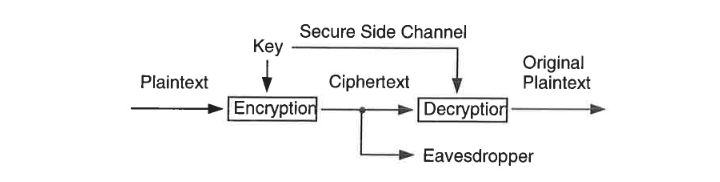
\includegraphics[width=\linewidth]{../pictures/simple_WEP_schema.PNG}
	\caption{Simples esquema de cifragem da mensagem utilizado pelo WEP. Fonte [1].}
	\label{fig:wep_schema}
\end{figure}

As especificações mais detalhadas e sua implementação podem ser encontradas em [1].

\subsubsection{WPA}
WPA era uma solução intermediária para a melhoria dos padrões de segurança estabelecidos anteriormente. Porém, WPA demonstrou vulnerabilidades significativas e foi posteriormente substituído pela sua segunda versão, WPA2. \par
Ambos WPA e WPA2 utilizam o mesmo método de autenticação, porém utilizam diferentes métodos de criptografia e algoritmos de integridade de dados. Redes corporativas utilizam frameworks \textbf{802.1 X/EAP} para sistemas centralizados de autenticação mútua, enquanto que redes pequenas e domésticas utilizam o \textbf{PSK} (Pré-Shared Key).\par
Na figura 2, vista abaixo, pode-se verificar uma comparação entre os \textit{Throughputs} de redes que utilizam nenhum método de segurança, WPA e WPA2, respectivamente. \par

%Imagem
\begin{figure}[h!]
	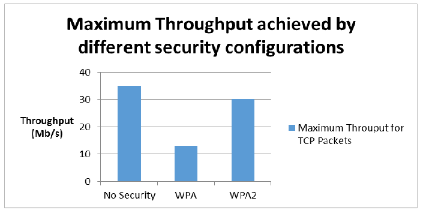
\includegraphics[width=\linewidth]{../pictures/throughput.PNG}
	\caption{Comparativo de 'throughput' de diferentes métodos de segurança. Fonte [2].}
	\label{fig:throughput_wpa}
\end{figure}

\subsection{Ataques à redes Wi-Fi usando o aircrack-ng}
Foi providenciado um dispositivo de ponto de acesso para a parte prática desse experimento, dispositivo no qual foi configurado com SSID 'seguranca' e método de segurança WEP, como mostra a figura 3 abaixo.
\vfill

%figura 3
\begin{figure}[h!]
	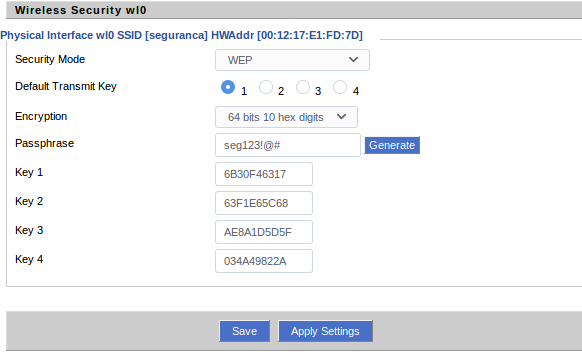
\includegraphics[width=\linewidth]{../pictures/WEP_passphrase.png}
	\caption{Configuração feita no AP e demonstração de como funciona o WEP.}
	\label{fig:WEP}
\end{figure}

\subsubsection{Descobrindo o SSID}
Simulando um atacante, que de antemão não tem conhecimento algum sobre as redes wi-fi que estão ali presentes, deve-se descobrir o SSID da rede que será atacada, é utilizado então o wireshark (ou qualquer outro software '\textit{sniffer}') e espera-se pacotes de '\textit{Beacon}', que são pacotes de varredura e possuem informações sobre a rede 802.11.\par
Na figura 5, no final do relatório, é mostrado um exemplo de um pacote capturado quando é utilizada a interface de rede em modo 'monitor', ou promíscuo. Nele se encontram informações valiosas que qualquer um pode ver, tais como, endereço MAC dos dispositivos envolvidos e seus respectivos fabricantes, SSID da rede, banda de frequência utilizada, taxas de transmissão, entre outras.



\subsubsection{Captura de pacotes}
Agora, utilizando o modo promíscuo e a ferramenta airocrack-ng, capturam-se os pacotes trafegados no meio que contenham endereço MAC do AP que já é sabido pelo atacante. Foi utilizado o comando como super usuário:
\begin{lstlisting}[language=Bash]
# airodump-ng -c 6 --bssid 
> 00:12:17:e1:fd:7d -w capture mon0
\end{lstlisting}

Dessa maneira, foi possível entrar em um modo onde o programa está rodando e é possível verificar várias informações sobre a captura, como mostra a figura 4 abaixo.

%figura 4
\begin{figure}[h!]
	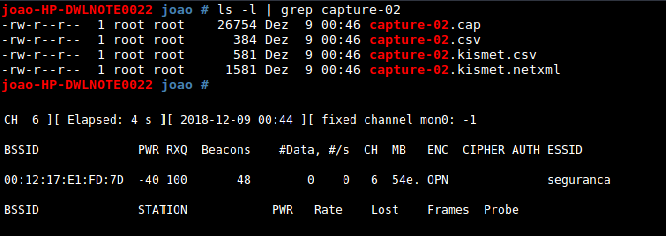
\includegraphics[width=\linewidth]{../pictures/airocrack_running+pcaps.png}
	\caption{Airodump rodando e seus arquivos de saída.}
	\label{fig:airodump}
\end{figure}


\section{Conclusão}
Primeiramente, o mais importante a se ressaltar é que deve-se tomar um cuidado extra ao se conectar em redes wifi públicas, já que seu dispositivos ficará exposto, e por consequência, suas informações mais valiosas e privadas. \par
Caso seja de extrema importância se conectar a uma rede pública e insegura - como, a de um aeroporto, por exemplo - uma boa escolha seria a utilização de uma VPN, fazendo com que o seu tráfego de rede seja totalmente cifrado, e assim, seguro.\par

%figura 5 pacote + modo monitor
\begin{figure*}[t!]
	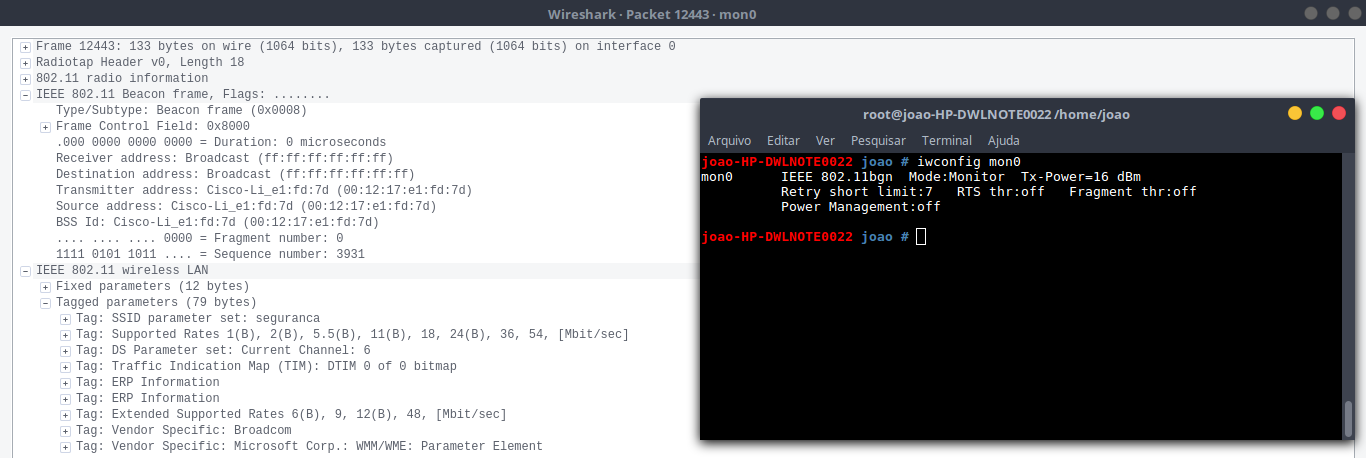
\includegraphics[width=\linewidth]{../pictures/monitor_mode_packet.png}
	\caption{Exemplo de pacote capturado e modo monitor ativado.}
	\label{fig:packet}
\end{figure*}

\begin{thebibliography}{1}

\bibitem{WEP}
\url{http://www.ieee802.org/11/Documents/DocumentArchives/1994_docs/1194249_scan.pdf}
\bibitem{Comparative}
A comparative study of WLAN security protocols: WPA, WPA2 \\
\url{https://ieeexplore.ieee.org/document/7506822}



\end{thebibliography}



\end{document}


